\documentclass[english,,man]{apa6}
\usepackage{lmodern}
\usepackage{amssymb,amsmath}
\usepackage{ifxetex,ifluatex}
\usepackage{fixltx2e} % provides \textsubscript
\ifnum 0\ifxetex 1\fi\ifluatex 1\fi=0 % if pdftex
  \usepackage[T1]{fontenc}
  \usepackage[utf8]{inputenc}
\else % if luatex or xelatex
  \ifxetex
    \usepackage{mathspec}
  \else
    \usepackage{fontspec}
  \fi
  \defaultfontfeatures{Ligatures=TeX,Scale=MatchLowercase}
\fi
% use upquote if available, for straight quotes in verbatim environments
\IfFileExists{upquote.sty}{\usepackage{upquote}}{}
% use microtype if available
\IfFileExists{microtype.sty}{%
\usepackage{microtype}
\UseMicrotypeSet[protrusion]{basicmath} % disable protrusion for tt fonts
}{}
\usepackage{hyperref}
\PassOptionsToPackage{usenames,dvipsnames}{color} % color is loaded by hyperref
\hypersetup{unicode=true,
            pdftitle={Evolution of Statistical Software and Quantitative Methods},
            pdfauthor={Brandon LeBeau~\& Ariel M. Aloe},
            pdfkeywords={Research Synthesis, Statistical Software, Quantitative Methods},
            colorlinks=true,
            linkcolor=blue,
            citecolor=Blue,
            urlcolor=Blue,
            breaklinks=true}
\urlstyle{same}  % don't use monospace font for urls
\ifnum 0\ifxetex 1\fi\ifluatex 1\fi=0 % if pdftex
  \usepackage[shorthands=off,main=english]{babel}
\else
  \usepackage{polyglossia}
  \setmainlanguage[]{english}
\fi
\usepackage{longtable,booktabs}
\usepackage{graphicx,grffile}
\makeatletter
\def\maxwidth{\ifdim\Gin@nat@width>\linewidth\linewidth\else\Gin@nat@width\fi}
\def\maxheight{\ifdim\Gin@nat@height>\textheight\textheight\else\Gin@nat@height\fi}
\makeatother
% Scale images if necessary, so that they will not overflow the page
% margins by default, and it is still possible to overwrite the defaults
% using explicit options in \includegraphics[width, height, ...]{}
\setkeys{Gin}{width=\maxwidth,height=\maxheight,keepaspectratio}
\IfFileExists{parskip.sty}{%
\usepackage{parskip}
}{% else
\setlength{\parindent}{0pt}
\setlength{\parskip}{6pt plus 2pt minus 1pt}
}
\setlength{\emergencystretch}{3em}  % prevent overfull lines
\providecommand{\tightlist}{%
  \setlength{\itemsep}{0pt}\setlength{\parskip}{0pt}}
\setcounter{secnumdepth}{0}
% Redefines (sub)paragraphs to behave more like sections
\ifx\paragraph\undefined\else
\let\oldparagraph\paragraph
\renewcommand{\paragraph}[1]{\oldparagraph{#1}\mbox{}}
\fi
\ifx\subparagraph\undefined\else
\let\oldsubparagraph\subparagraph
\renewcommand{\subparagraph}[1]{\oldsubparagraph{#1}\mbox{}}
\fi

%%% Use protect on footnotes to avoid problems with footnotes in titles
\let\rmarkdownfootnote\footnote%
\def\footnote{\protect\rmarkdownfootnote}


  \title{Evolution of Statistical Software and Quantitative Methods}
    \author{Brandon LeBeau\textsuperscript{1}~\& Ariel M. Aloe\textsuperscript{1}}
    \date{}
  
\shorttitle{Evolution Software and Methods}
\affiliation{
\vspace{0.5cm}
\textsuperscript{1} University of Iowa}
\keywords{Research Synthesis, Statistical Software, Quantitative Methods}
\usepackage{csquotes}
\usepackage{upgreek}
\captionsetup{font=singlespacing,justification=justified}

\usepackage{longtable}
\usepackage{lscape}
\usepackage{multirow}
\usepackage{tabularx}
\usepackage[flushleft]{threeparttable}
\usepackage{threeparttablex}

\newenvironment{lltable}{\begin{landscape}\begin{center}\begin{ThreePartTable}}{\end{ThreePartTable}\end{center}\end{landscape}}

\makeatletter
\newcommand\LastLTentrywidth{1em}
\newlength\longtablewidth
\setlength{\longtablewidth}{1in}
\newcommand{\getlongtablewidth}{\begingroup \ifcsname LT@\roman{LT@tables}\endcsname \global\longtablewidth=0pt \renewcommand{\LT@entry}[2]{\global\advance\longtablewidth by ##2\relax\gdef\LastLTentrywidth{##2}}\@nameuse{LT@\roman{LT@tables}} \fi \endgroup}


\DeclareDelayedFloatFlavor{ThreePartTable}{table}
\DeclareDelayedFloatFlavor{lltable}{table}
\DeclareDelayedFloatFlavor*{longtable}{table}
\makeatletter
\renewcommand{\efloat@iwrite}[1]{\immediate\expandafter\protected@write\csname efloat@post#1\endcsname{}}
\makeatother

\authornote{

Correspondence concerning this article should be addressed to Brandon
LeBeau, Psychological and Quantitative Foundations, University of Iowa,
Iowa City, IA 52245. E-mail:
\href{mailto:brandon-lebeau@uiowa.edu}{\nolinkurl{brandon-lebeau@uiowa.edu}}}

\abstract{
Statistical software is the enabling tool of quantitative research
studies and the availability and use of the software can greatly shape
which methods are used by researchers. Software that is more accessible
is likely to have more users and the methods implemented within the
software limits the methods accessible to researchers. Open source
software, (e.g.~R), has reduced these barriers by making cutting edge
statistical methods available to researchers through add-on packages.
This paper aims to explore the evolution of statistical software within
social science research using a research synthesis to establish the
state of affairs.


}

\usepackage{amsthm}
\newtheorem{theorem}{Theorem}[section]
\newtheorem{lemma}{Lemma}[section]
\theoremstyle{definition}
\newtheorem{definition}{Definition}[section]
\newtheorem{corollary}{Corollary}[section]
\newtheorem{proposition}{Proposition}[section]
\theoremstyle{definition}
\newtheorem{example}{Example}[section]
\theoremstyle{definition}
\newtheorem{exercise}{Exercise}[section]
\theoremstyle{remark}
\newtheorem*{remark}{Remark}
\newtheorem*{solution}{Solution}
\begin{document}
\maketitle

\hypertarget{objectives}{%
\section{Objectives}\label{objectives}}

The purpose of this paper is to explore the evolution (or lack thereof)
of statistical software usage over time in education. As this usage is
likely tied closely to the methods they are employed, the interaction
between software usage and quantitative research methods will also be
explored. Research synthesis methods (Cooper, 2016) will be used to
explore these trends over time in published social science research
journals.

\hypertarget{theoretical-framework}{%
\section{Theoretical Framework}\label{theoretical-framework}}

Statistical software is the enabling tool to performing applied data
analysis. Statistical methods that are implemented within software will
increase their usage (particularly if the software is also
user-friendly) by applied analysts and are likely taught more frequently
in methodology courses at universities. Moreover, casual users of
statistics software may not distinguish between the limitations of the
models and the limitations of the software. In addition, the
user-friendly nature of software (i.e., point and click graphical
interfaces, ability to manipulate data by hand) also can severely limit
the ability for research to be reproducible; a recent topic of intense
discussion in biostatistics, medicine, and pyschology (Asendorpf et al.,
2013; Ioannidis, 2014; Iqbal, Wallach, Khoury, Schully, \& Ioannidis,
2016; Peng, 2009, 2011; Stodden, 2012). The reproducibility crisis has
pointed the finger at statistical software more directly with a strong
push in some disciplines for analyses to be script (i.e., source code)
based and posted with the published journal article, often described as
the gold standard.

This idea of reproducibility has not seemed to fully enter the social
science research domain. SPSS is likely the most common statistical
software program used in many social science research domains,
particularly education. Although SPSS has many common and advanced
statistical techniques and it is possible to have a reproducible
analysis, the default behavior within this program is often not script
based and can create bad habits (i.e., editing raw data directly in the
gui interface, running analyses without saving a script, etc.).
Statistical software that is primarily command line, programs such as R
or Python, offer easier reproducible frameworks as all data
manipulations or analyses are saved in scripts that can be re-ran in the
future. A data script can be thought of as a cockpit flight recorder in
which every single step that was done to the original data going from
data collection to final tables and figures was script based. Under a
reproducible framework, the raw data are never altered directly, they
should always be altered programmatically through a script. This keeps a
log of the data manipulations that happened in the data analysis cycle.
For example, R has packages that aid in the ability to create living
data documents that contain text and analysis code within a single
document (see Allaire et al., 2017; Xie, 2015, 2017).

The reproducible analysis framework has many advantages, including a
transparent analysis process that could be validated by others or even
simply the ability to investigate the data analysis completed months or
years previously. Unfortunately, the current academic research framework
has many barriers that limit the reproducibility. First, applied
researchers may not be users of primarily command line or script based
statistical software. This limits the ability to create a reproducible
framework from the start. Secondly, researchers are not incentivized to
conduct an analysis in a reproducible framework. Namely, the publish or
perish aspect of academic research limits the sharing of statistical
code partly due to the increased chance of criticism upon evaluation of
the code used for the analysis. Finally, many journals and even the
American Psychological Association (APA) publication manual (American
Psychological Association, 2010) states that common software or
programming languages need not be cited. This could even be interpretted
by some as not needing to mention. Unfortunately, if the software used
for a data analysis is not reported, the ability to recreate the
analysis drops even more due to differences in estimation, handling of
missing data, or other software specific settings.

This paper aims to explore the state of affairs in statistical software
usage in education. Particular attention will be made to which software
is currently being used in published social science research as well as
how this has changed over the last twenty years. Secondly, this paper
also aims to explore how frequently open-source software tools are used
and to explore evidence of reproducible analysis framework being
implemented. These aims will be explored using research synthesis
methods.

\hypertarget{research-questions}{%
\subsection{Research Questions}\label{research-questions}}

\begin{enumerate}
\def\labelenumi{\arabic{enumi}.}
\tightlist
\item
  To what extent has the statistical software usage shifted over time in
  published analyses?

  \begin{itemize}
  \tightlist
  \item
    If there is evidence of a shift, is there evidence this shift
    differs based on quantitative method or journal?
  \end{itemize}
\item
  To what extent are published analyses citing statistical software?

  \begin{itemize}
  \tightlist
  \item
    Has this changed over time and across journals?
  \end{itemize}
\item
  To what extent are open-source software tools used?

  \begin{itemize}
  \tightlist
  \item
    Is there evidence of reproducible analyses being employed?
  \end{itemize}
\end{enumerate}

\hypertarget{methods}{%
\section{Methods}\label{methods}}

Research synthesis methods (Cooper, 2016) will be used to explore the
evolution of statistical software and quantitative methods in social
science research. More specifically, the statistical software used for
the analysis will be coded in additional to the specific quantitative
methods (i.e.~linear regression, hierarchical linear model, etc.).
Additional meta data will also be coded including, journal, article
title, author information, article keywords, year published, and any
mention of supplementary materials. This information will be used to
explore descriptive trends in the data over time, by journals, and
methods.

The research synthesis will gather data from a handful of education
journals that primarily publish empirical data analysis. The search will
not include journals that the primary focus is methodological, the use
of software in these journals would likely be a different population
than those that are data analytic in nature. Therefore the following
journals were selected to be searched from 1995 onward:

\begin{itemize}
\tightlist
\item
  American Economic Journal (AEJ)
\item
  American Educational Research Journal (AERJ)
\item
  American Journal of Political Science (AJPS)
\item
  Economic Journal (EJ)
\item
  Educational Evaluation and Policy Analysis (EEPA)
\item
  Educational Researcher (ER)
\item
  Higher Education (HE)
\item
  Journal of Experimental Education (JEE)
\item
  Journal of Public Policy (JPP)
\item
  Political Science Quarterly (PSQ)
\item
  Public Policy Administration (PPA)
\item
  Sociology of Education (SE)
\end{itemize}

\hypertarget{data-and-software}{%
\subsection{Data and Software}\label{data-and-software}}

All journal articles published between 1995 through the middle of 2018
will be organized into EndNote. Within EndNote, the find pdf feature
will be used to gather the published documents from each journal. This
pdf database will then be searched using the \emph{pdfsearch} R package
(LeBeau, 2018; R Core Team, 2017). This package allows for keyword
searching directly within pdf documents. This will be the primary data
collection method. The software keywords searched for can be seen in
Table \ref{tab:searchwords}. Table \ref{tab:searchwords} also shows
keywords to be used to search for statistical models and estimation
methods. A handful of articles will be randomly selected to be coded
manually by reading the document to evaluate the accuracy of coding
using the \emph{pdfsearch} package.

Additional metadata obtained from journal articles will be obtained and
combined with the keyword searching data. This metadata will contain
information such as, year of publication, publication keywords, author
information, and other article metadata obtained from EndNote. These
data will be used to further enhance the keyword search data obtained
from the \emph{pdfsearch} package and the subsequent analyses discussed
in the next section.

\begin{longtable}[]{@{}lll@{}}
\caption{\label{tab:searchwords} Search keywords used in search of published
journal documents}\tabularnewline
\toprule
\begin{minipage}[b]{0.20\columnwidth}\raggedright
Search\strut
\end{minipage} & \begin{minipage}[b]{0.10\columnwidth}\raggedright
Group\strut
\end{minipage} & \begin{minipage}[b]{0.37\columnwidth}\raggedright
Keywords\strut
\end{minipage}\tabularnewline
\midrule
\endfirsthead
\toprule
\begin{minipage}[b]{0.20\columnwidth}\raggedright
Search\strut
\end{minipage} & \begin{minipage}[b]{0.10\columnwidth}\raggedright
Group\strut
\end{minipage} & \begin{minipage}[b]{0.37\columnwidth}\raggedright
Keywords\strut
\end{minipage}\tabularnewline
\midrule
\endhead
\begin{minipage}[t]{0.20\columnwidth}\raggedright
Software\strut
\end{minipage} & \begin{minipage}[t]{0.10\columnwidth}\raggedright
SPSS R SAS STATA Python Other HLM IRT Latent\strut
\end{minipage} & \begin{minipage}[t]{0.37\columnwidth}\raggedright
SPSS Statistics, SPSS Modeler, SPSS R-project, R Project, CRAN, R core
team, R software, RStudio SAS Insitute, SAS, JMP STATA \textbar{} Python
MATLAB, Statistica , Statsoft, Java, Hadoop, Minitab, Systat, Tableau,
Scala, Julia, Azure Machine Learning HLM{[}0-9{]}, HLM {[}0-9{]} BILOG,
BILOG-MG, Multilog, PARSCALE, IRT Pro Variable \textbar{} Mplus, LISREL,
AMOS\strut
\end{minipage}\tabularnewline
\begin{minipage}[t]{0.20\columnwidth}\raggedright
Statistical Models\strut
\end{minipage} & \begin{minipage}[t]{0.10\columnwidth}\raggedright
ANOVA HLM \textbar{} H Latent t-test Regress Growth Other\strut
\end{minipage} & \begin{minipage}[t]{0.37\columnwidth}\raggedright
Analysis of Variance, ANOVA, ANCOVA, Analysis of Covariance,
multivariate analysis of variance, MANOVA, repeated measures analysis of
variance, RMANOVA, RM-ANOVA LM, Hierarchical Linear Model, Linear Mixed
Model, LMM, Multilevel Model, Multi-level Model Variable \textbar{} item
response theory, IRT, confirmatory factor analysis, CFA, exploratory
factor analysis, EFA, latent variable modeling, structural equation
modeling, SEM \textbar{} one sample t-test, one-sample t-test, two
sample t-test, two-sample t-test, dependent samples t-test,
dependent-sample t-test ion \textbar{} Regression, multiple regression,
linear regression, multiple linear regression, nonlinear regression,
non-linear regression, logistic regression, ordinal regression,
multinomial logistic regression, multinomial regression, generalized
additive models, GAM, general(ized)? linear model, general(ized)? linear
mixed model \textbar{} growth model, latent growth model, LGM cluster
analysis, hierarchical cluster analysis, propensity score matching,
propensity score analysis, meta analysis, meta-analysis, nonparametric
analysis, chi-square( analysis)?\strut
\end{minipage}\tabularnewline
\bottomrule
\end{longtable}

\hypertarget{analysis}{%
\subsection{Analysis}\label{analysis}}

Descriptive analyses will be performed on the research synthesis data
obtained from keyword searching performed with the \emph{pdfsearch}
package. Initial exploration will focus on software and statistical
models separately. Subsequent descriptive analyses will be performed to
explore the if there are any intereactions between software and
statistical models used in published research. All of these analyses
will be performed over time to explore trends in software and
statistical model usage and citation rates. Figures will be the primary
analysis methods and will be created in R using the ggplot2 package
(Wickham, 2016).

\hypertarget{results}{%
\section{Results}\label{results}}

The number and percentage of PDFs able to be obtained from EndNote is
shown in Table \ref{tab:setup}. Many of the journals had a high success
rate of obtaining the PDF for the published studies, however some were
problematic. For example, JPP and EEPA were both under 50\% of PDFs
obtained and AJPS, EJ, and SE were all just over 50\%. The PDFs that
were not obtained were attempted to be obtained over multiple occasions
over a six month period, with no additional PDFs obtained between the
last two attempts. Figure \ref{fig:pdf-time} shows the percentage of
PDFs obtained by year and journal and highlights some noticeable trends.
There are periods of time for specific journals that all the PDFs are
obtained compared to not obtained. For example, AJPS, EEPA, EJ, and SE
have periods from 1995 to just after 2000 where most of the PDFs were
not obtained. These ranges are portions of time in which our University
does not have digital access to these journals.

\begin{table}[!h]

\caption{\label{tab:setup}EndNote success rate of obtaining article PDf by journal.}
\centering
\begin{tabular}[t]{lrrr}
\toprule
Journal & Number of PDFs & Total Possible Articles & Percent PDFs Obtained\\
\midrule
AEJ & 363 & 364 & 99.7\\
AERJ & 444 & 444 & 100.0\\
AJPS & 922 & 1436 & 64.2\\
EEPA & 188 & 405 & 46.4\\
EJ & 1829 & 3376 & 54.2\\
\addlinespace
ER & 742 & 794 & 93.5\\
HE & 1914 & 1914 & 100.0\\
JEE & 517 & 525 & 98.5\\
PSQ & 2722 & 3589 & 75.8\\
PPA & 83 & 83 & 100.0\\
\addlinespace
JPP & 27 & 180 & 15.0\\
SE & 261 & 453 & 57.6\\
\bottomrule
\end{tabular}
\end{table}

\begin{figure}
\centering
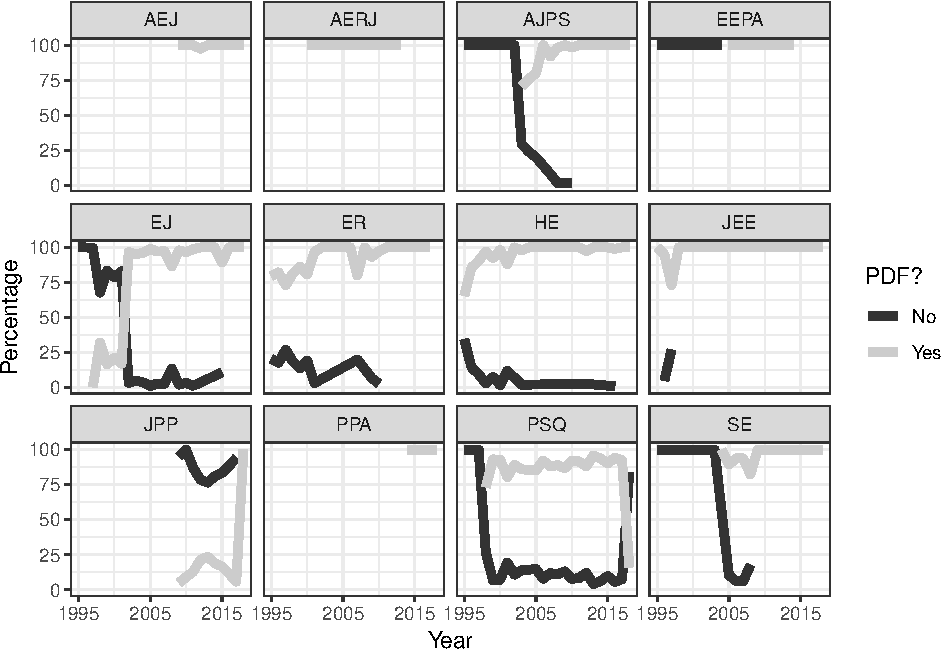
\includegraphics{software_files/figure-latex/pdf-time-1.pdf}
\caption{\label{fig:pdf-time}Number of PDFs obtained by journal and year.}
\end{figure}

Using the obtained PDFs, keyword searching was performed for the
software and model keywords. Figure \ref{fig:count-software} shows the
percentage of articles from each journal with at least one match for
software and model keywords. A few trends emerge from this figure.
First, software keywords are much less likely to be found within the
obtained PDFs. The largest percentage was in JEE with about 50\% of
obtained articles reporting at least one of the searched software
keywords. Most of the other journals only had 25\% or less of the
articles mentioning one of the software keywords, with none of the
obtained articles in JPP mentioning a software keyword. Model keywords
on the other hand were much better more prevalent and the journals fall
into two broad groups. One group, JEE, EEPA, AEJ, AJPS, SE, and EJ have
more than 50\% of the obtained articles mentioning at least one of the
model keywords and the remaining journals being less than 50\%. The
articles in the latter group, with the exception of AERJ, were closer to
25\% of less.

\begin{figure}
\centering
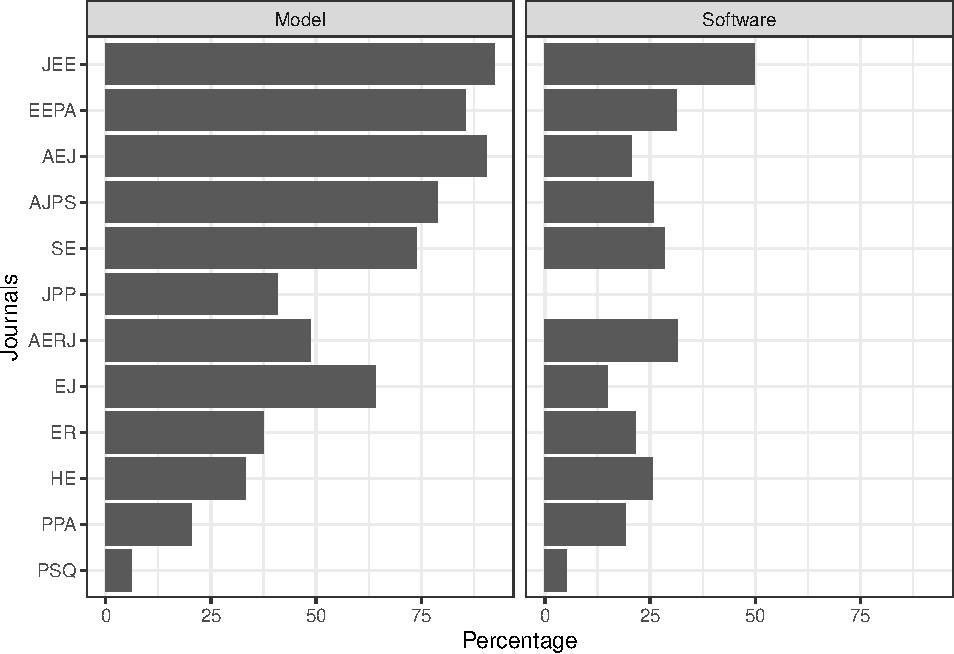
\includegraphics{software_files/figure-latex/count-software-1.pdf}
\caption{\label{fig:count-software}Number of articles with at least one
model or software keyword match by journals.}
\end{figure}

\begin{figure}
\centering
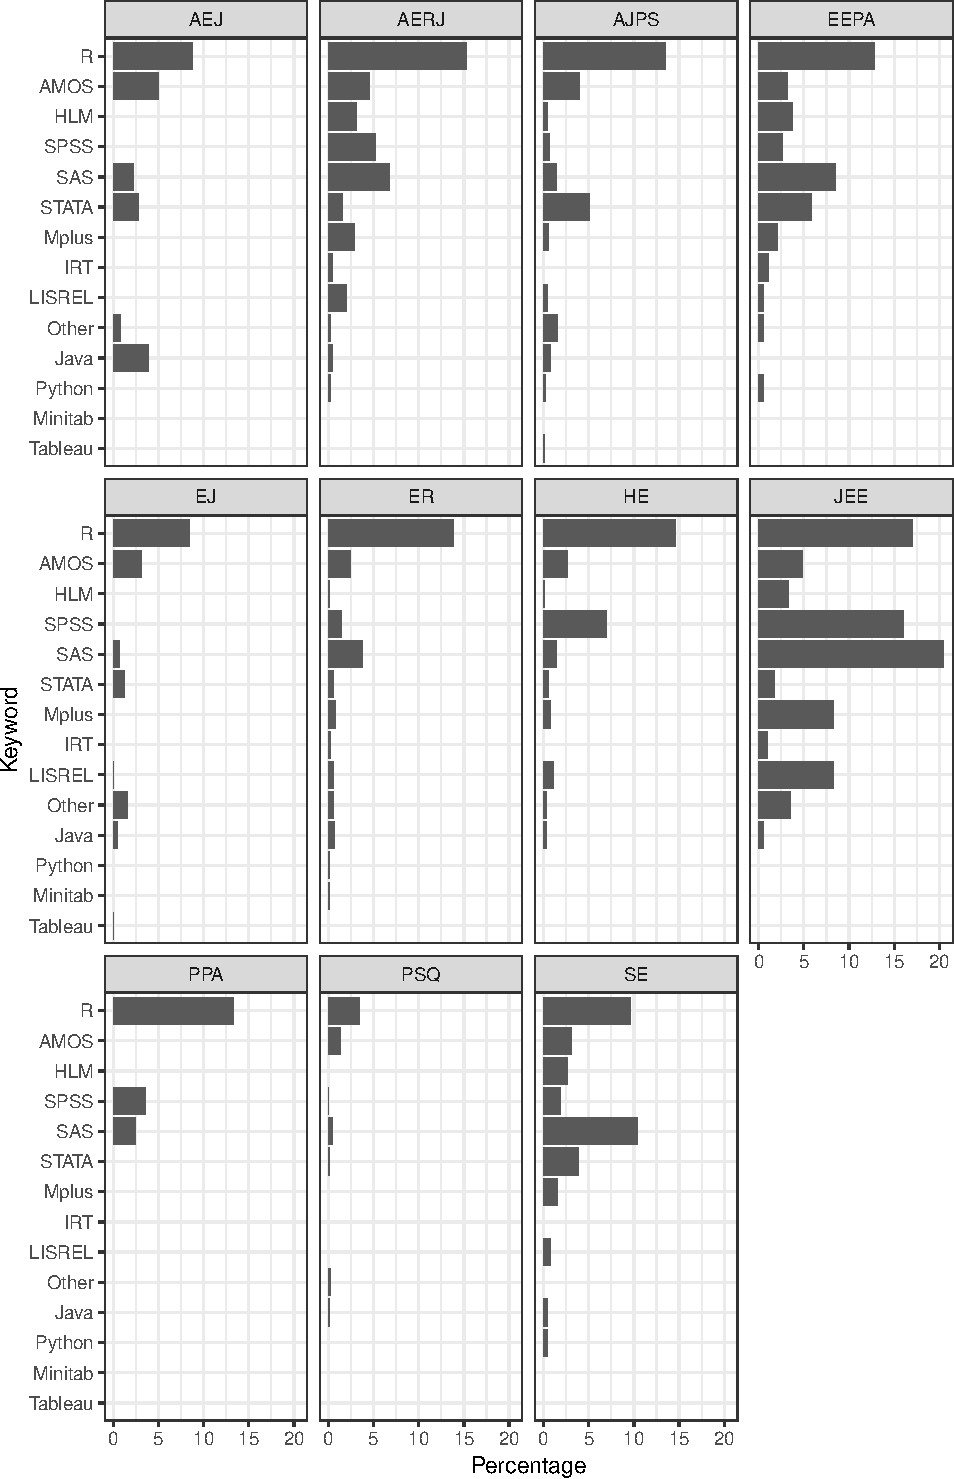
\includegraphics{software_files/figure-latex/software-journal-1.pdf}
\caption{\label{fig:software-journal}Software counts by journal}
\end{figure}

Expanding on the software keywords found within the PDFs, Figure
\ref{fig:software-journal} explores which software keywords were found
in each journal. In general, mirroring results from Figure
\ref{fig:count-software}, the percetage of articles reporting software
keywords was relatively small, most often less than 5\%. R, SAS, SPSS,
and STATA were the most commonly found software keywords, with R being
the most common in most journals. The one exception to this was in JEE,
where SAS was more common (about 20\% of articles) and R and SPSS had a
similar percentage (about 15\%) of articles reporting their usage. One
interpretation note, articles may mention more than one software keyword
and those duplicate results will show up in each category. On average,
the average number of software keywords identified in each article was
highest for JEE at 1.71 (range: 1 to 5) and a lowest of 1 for PPA
(range: 1 to 1).

A similar figure for model keywords can be seen in Figure
\ref{fig:model-journal}. The x-axis scale here is wider compared to the
software keywords showing that the methods are more commonly reported.
However, there are still a sizeable number of articles appearing in
these journals that do not list one of the model keywords searched. The
most commonly used methods are linear model, analysis of variance,
meta-analysis, or linear mixed model (i.e.~HLM) models. The journals
EEPA, JEE, and SE have the widest array of models being picked up
through the keyword search. On the opposite side, AEJ, AJPS, and EJ are
dominated by linear models. Finally, journals such as AERJ, ER, HE, PPA,
and PSQ all have a low prevalence of articles that are using the model
keywords.

\begin{figure}
\centering
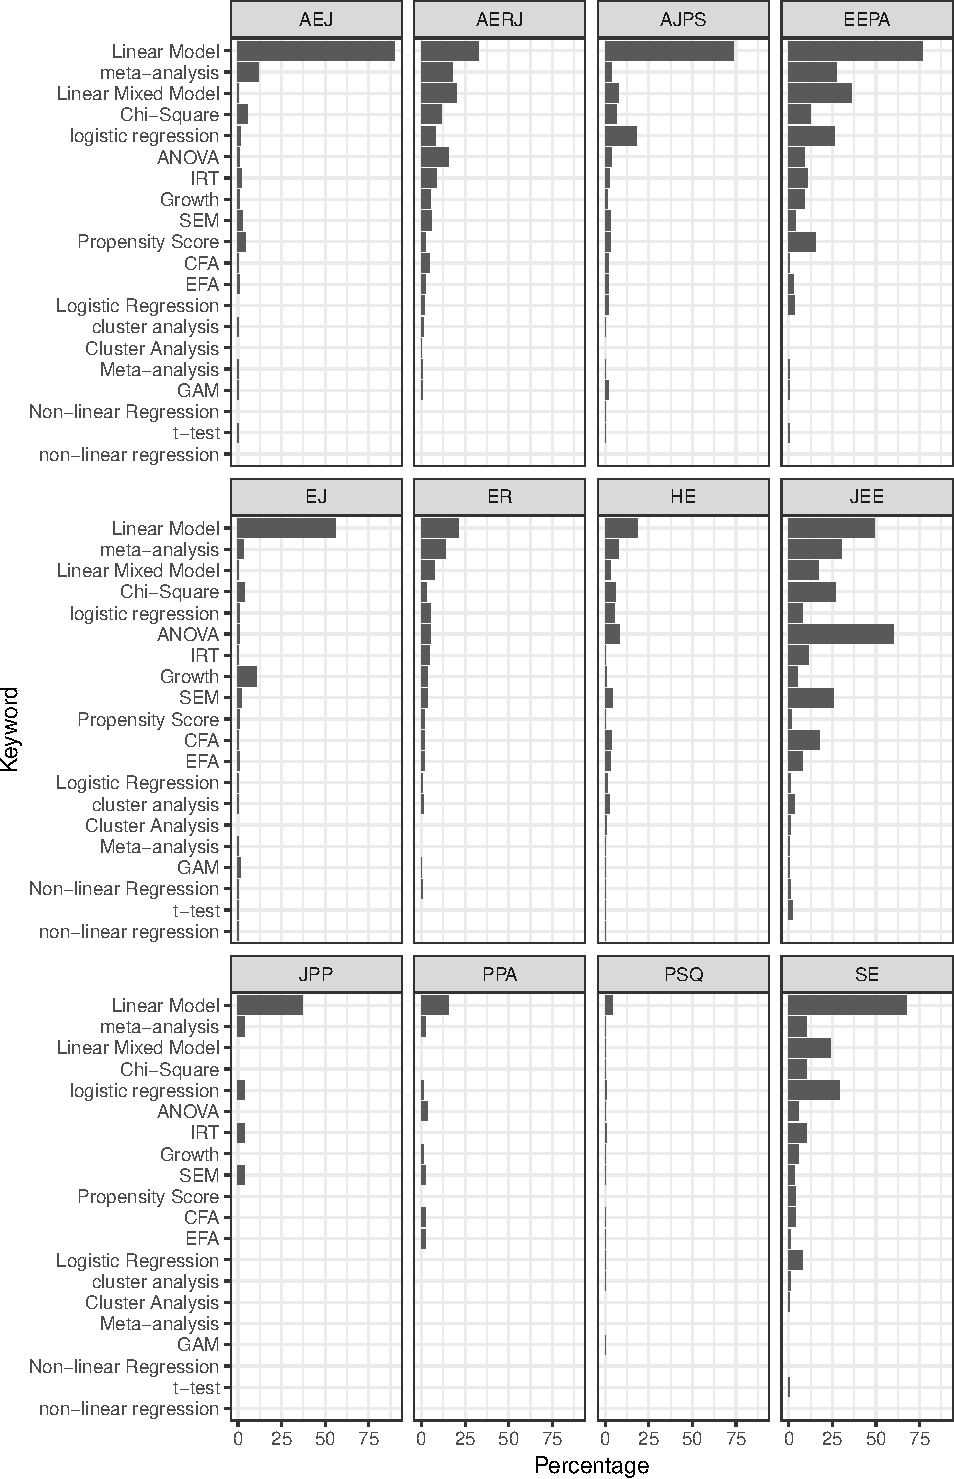
\includegraphics{software_files/figure-latex/model-journal-1.pdf}
\caption{\label{fig:model-journal}Statistical Model counts by journal}
\end{figure}

\hypertarget{interaction-between-software-and-statistical-methods}{%
\subsection{Interaction between software and statistical
methods}\label{interaction-between-software-and-statistical-methods}}

\hypertarget{discussion}{%
\section{Discussion}\label{discussion}}

\hypertarget{references}{%
\section{References}\label{references}}

\setlength{\parindent}{-0.5in}
\setlength{\leftskip}{0.5in}

\begin{figure}
\centering
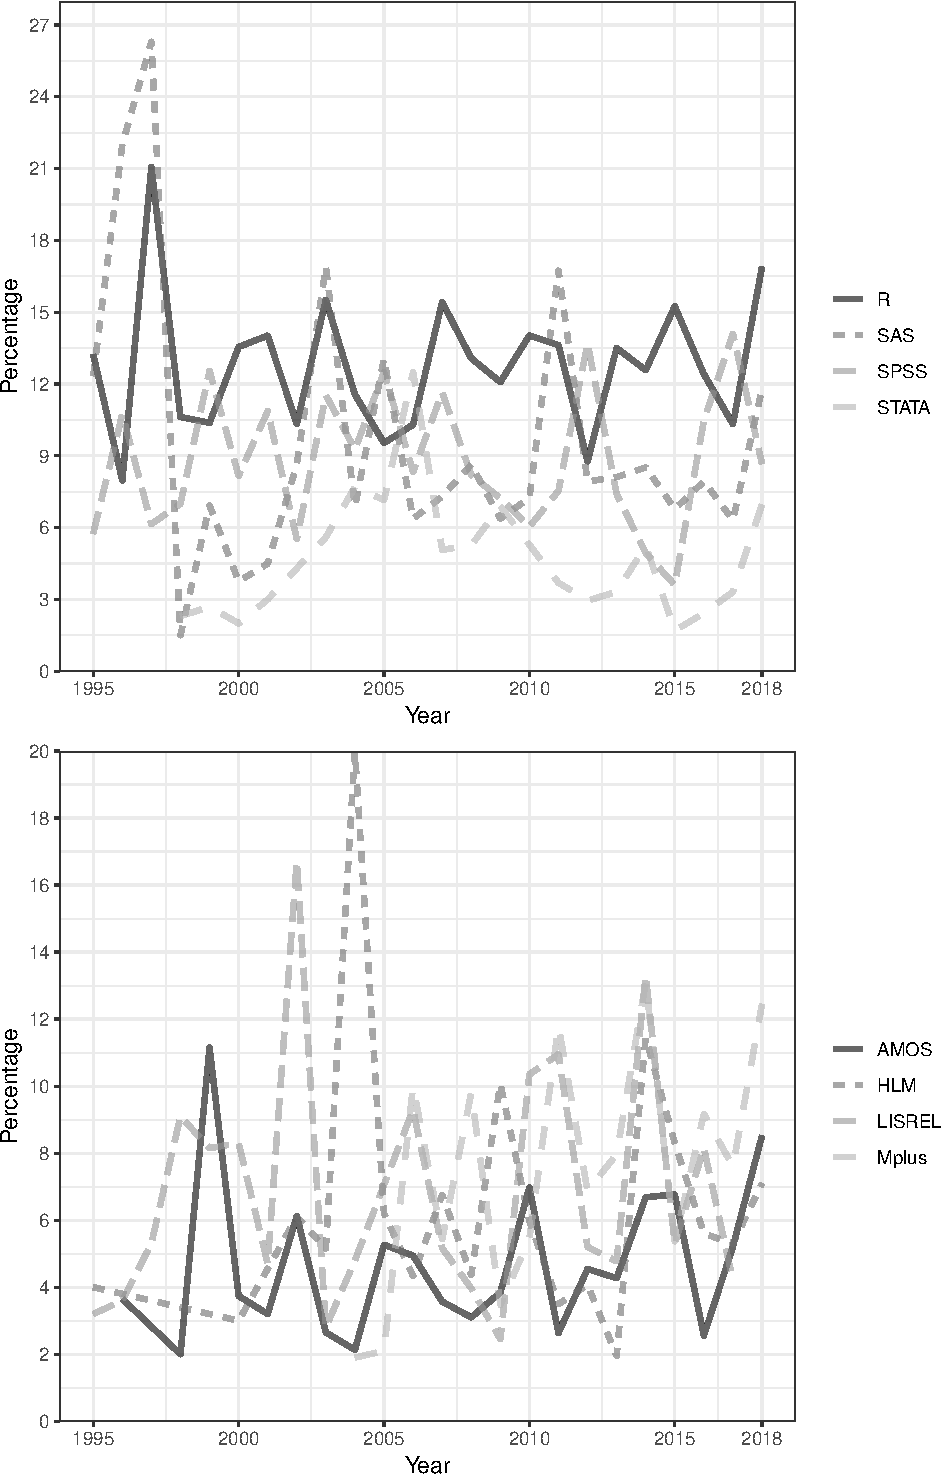
\includegraphics{software_files/figure-latex/software-year-at1-1.pdf}
\caption{\label{fig:software-year-at1}Software percentages by year}
\end{figure}

\begin{figure}
\centering
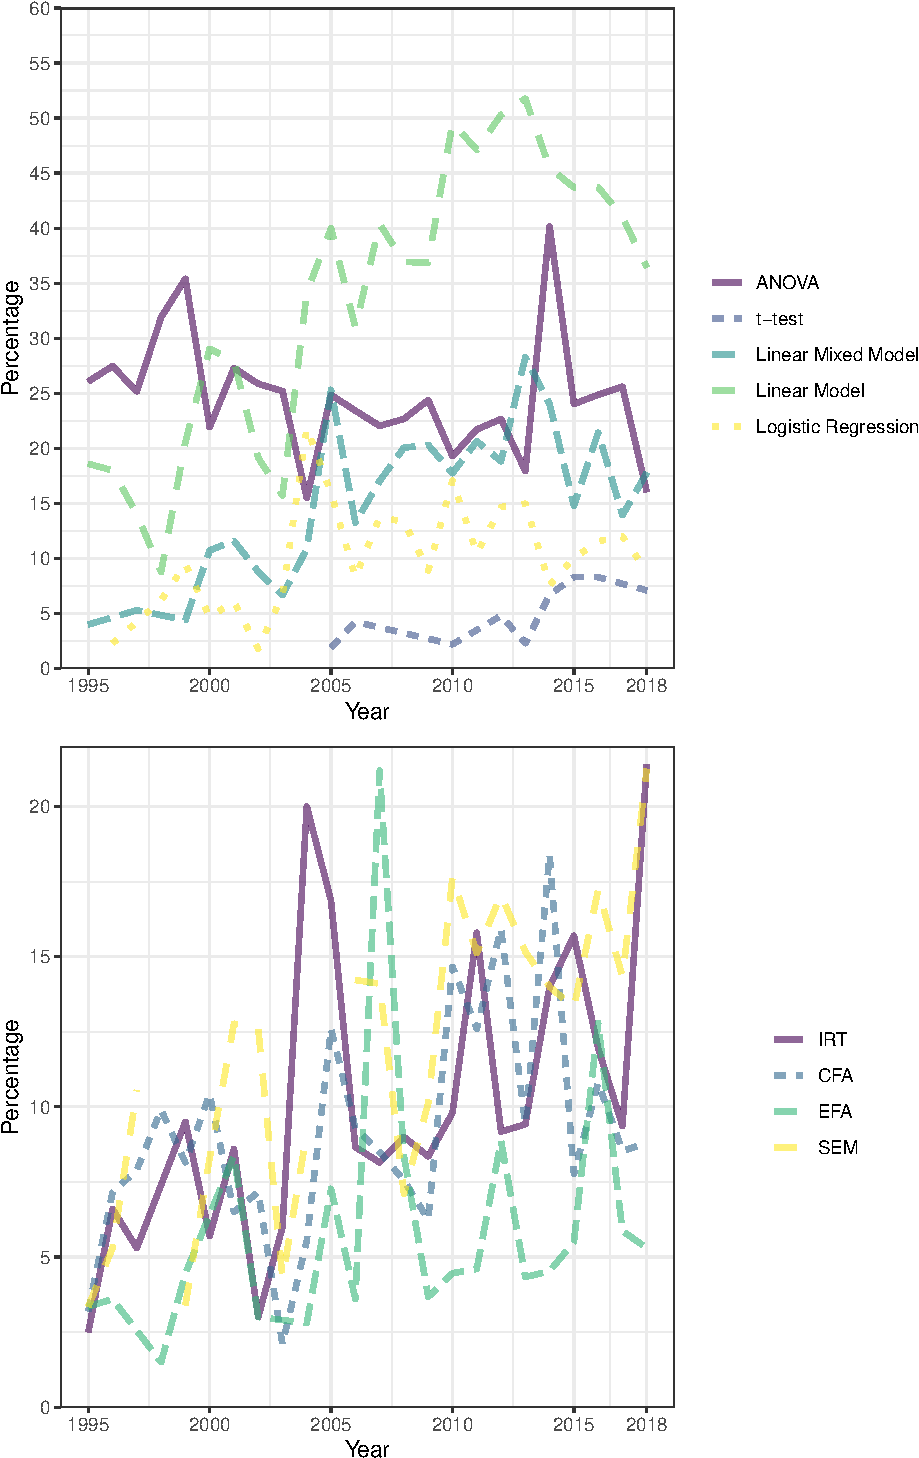
\includegraphics{software_files/figure-latex/model-year-at1-1.pdf}
\caption{\label{fig:model-year-at1}Model percentages by year}
\end{figure}

\hypertarget{refs}{}
\leavevmode\hypertarget{ref-rmarkdown}{}%
Allaire, J., Cheng, J., Xie, Y., McPherson, J., Chang, W., Allen, J.,
\ldots{} Arslan, R. (2017). \emph{Rmarkdown: Dynamic documents for r}.
Retrieved from \url{https://CRAN.R-project.org/package=rmarkdown}

\leavevmode\hypertarget{ref-apa}{}%
American Psychological Association. (2010). \emph{Publication manual of
the american psychological association}. Washington, D.C.: American
Psychological Association.

\leavevmode\hypertarget{ref-asendorpf2013}{}%
Asendorpf, J. B., Conner, M., De Fruyt, F., De Houwer, J., Denissen, J.
J., Fiedler, K., \ldots{} others. (2013). Recommendations for increasing
replicability in psychology. \emph{European Journal of Personality},
\emph{27}(2), 108--119.

\leavevmode\hypertarget{ref-cooper2016}{}%
Cooper, H. (2016). \emph{Research synthesis and meta-analysis: A
step-by-step approach} (Vol. 2). Sage publications.

\leavevmode\hypertarget{ref-ioannidis2014}{}%
Ioannidis, J. P. (2014). How to make more published research true.
\emph{PLoS Medicine}, \emph{11}(10), e1001747.

\leavevmode\hypertarget{ref-iqbal2016}{}%
Iqbal, S. A., Wallach, J. D., Khoury, M. J., Schully, S. D., \&
Ioannidis, J. P. (2016). Reproducible research practices and
transparency across the biomedical literature. \emph{PLoS Biology},
\emph{14}(1), e1002333.

\leavevmode\hypertarget{ref-pdfsearch}{}%
LeBeau, B. (2018). pdfsearch: Search tools for pdf files. \emph{Journal
of Open Source Software}, \emph{3}(27), 668.
doi:\href{https://doi.org/10.21105/joss.00668}{10.21105/joss.00668}

\leavevmode\hypertarget{ref-peng2009}{}%
Peng, R. D. (2009). Reproducible research and biostatistics.
\emph{Biostatistics}, \emph{10}(3), 405--408.
doi:\href{https://doi.org/10.1093/biostatistics/kxp014}{10.1093/biostatistics/kxp014}

\leavevmode\hypertarget{ref-peng2011}{}%
Peng, R. D. (2011). Reproducible research in computational science.
\emph{Science}, \emph{334}(6060), 1226--1227.

\leavevmode\hypertarget{ref-rpro}{}%
R Core Team. (2017). \emph{R: A language and environment for statistical
computing}. Vienna, Austria: R Foundation for Statistical Computing.
Retrieved from \url{https://www.R-project.org/}

\leavevmode\hypertarget{ref-stodden2012}{}%
Stodden, V. (2012). Reproducible research for scientific computing:
Tools and strategies for changing the culture. \emph{Computing in
Science \& Engineering}, \emph{14}(4), 13--17.

\leavevmode\hypertarget{ref-ggplot2}{}%
Wickham, H. (2016). \emph{Ggplot2: Elegant graphics for data analysis}.
Springer-Verlag New York. Retrieved from \url{http://ggplot2.org}

\leavevmode\hypertarget{ref-knitr}{}%
Xie, Y. (2015). \emph{Dynamic documents with R and knitr} (2nd ed.).
Boca Raton, Florida: Chapman; Hall/CRC. Retrieved from
\url{http://yihui.name/knitr/}

\leavevmode\hypertarget{ref-knitrmanual}{}%
Xie, Y. (2017). \emph{Knitr: A general-purpose package for dynamic
report generation in r}. Retrieved from \url{http://yihui.name/knitr/}


\end{document}
